\documentclass[11pt,a4paper]{article}

% --------------------------------------------------
% Packages
% --------------------------------------------------
\usepackage[utf8]{inputenc}
\usepackage[T1]{fontenc}
\usepackage{lmodern}
\usepackage{geometry}
\usepackage{setspace}
\usepackage{graphicx}
\usepackage{booktabs}
\usepackage{array}
\usepackage{longtable}
\usepackage{enumitem}
\usepackage{xcolor}
\usepackage{url}
\usepackage{amsmath}
\usepackage{amssymb}
\usepackage{float}
\usepackage{tikz}
\usepackage{listings}
\usepackage{fancyhdr}
\usepackage{titlesec}
\usepackage{caption}
\usepackage{tcolorbox}
\usepackage{hyperref}

\usetikzlibrary{
    positioning,
    arrows.meta,
    shapes.geometric,
    fit,
    backgrounds
}

% --------------------------------------------------
% Page Setup
% --------------------------------------------------
\geometry{
    left=20mm,
    right=20mm,
    top=25mm,
    bottom=25mm
}

\onehalfspacing
\setlength{\emergencystretch}{3em}

\hypersetup{
    colorlinks=true,
    linkcolor=teal!70!black,
    citecolor=teal!70!black,
    urlcolor=blue!70!black
}

% --------------------------------------------------
% Header & Footer
% --------------------------------------------------
\setlength{\headheight}{15pt}
\pagestyle{fancy}
\fancyhf{}
\lhead{\small\textbf{MASCV} --- Comprehensive System Documentation}
\rhead{\small Technical Reference}
\cfoot{\thepage}

% --------------------------------------------------
% Listings Style
% --------------------------------------------------
\definecolor{codebg}{rgb}{0.96,0.97,0.98}
\definecolor{codekw}{rgb}{0.13,0.29,0.53}
\definecolor{codestr}{rgb}{0.78,0.16,0.16}
\definecolor{codecomm}{rgb}{0.45,0.48,0.51}

\lstset{
    backgroundcolor=\color{codebg},
    basicstyle=\ttfamily\footnotesize,
    keywordstyle=\color{codekw}\bfseries,
    stringstyle=\color{codestr},
    commentstyle=\color{codecomm}\itshape,
    breaklines=true,
    breakatwhitespace=false,
    frame=single,
    rulecolor=\color{black!15},
    columns=fullflexible,
    keepspaces=true,
    showstringspaces=false
}

% --------------------------------------------------
% Custom Callout Box
% --------------------------------------------------
\newtcolorbox{agentbox}[2][]{
    colback=teal!5!white,
    colframe=teal!65!black,
    fonttitle=\bfseries\sffamily,
    title=#2,
    arc=2mm,
    boxrule=1pt,
    #1
}

% ==================================================
\begin{document}
% ==================================================

\begin{titlepage}
\centering
\vspace*{1.5cm}

{\huge\textbf{Multi-Agent Scientific Claim Verification System\\(MASCV)}}\\[0.6cm]
{\Large\textbf{Comprehensive Software Architecture \& Agent Specification Guide}}\\[0.4cm]
{\large An Evidence-Grounded Multi-Agent Framework for Adversarial Scientific Verification}

\vspace{1.5cm}
\begin{tcolorbox}[colback=blue!5!white,colframe=blue!60!black,arc=3mm,width=0.92\textwidth]
\centering
\textbf{Document Purpose:}\\[0.2cm]
\small
This technical documentation provides an exhaustive, file-by-file specification of the MASCV codebase. It details the theoretical motivation, input/output contracts, internal algorithms, configuration knobs, and file structure mapping for all seven specialized agents, the shared state machine, the RAG engine, and the evaluation suite.
\end{tcolorbox}

\vspace{1.5cm}
\begin{flushleft}
\textbf{Author / Primary Maintainer:} Beshoy Zaki\\
\textbf{Target Deployment:} Graduation Project / Research Publication\\
\textbf{Repository:} \url{https://github.com/Beshoy-Zaki/Multi-Agent-Scientific-Claim-Verification-System}\\
\textbf{Core Technologies:} Python 3.10+, LangGraph, Pydantic v2, Google Gemma 4 31B, arXiv API, Semantic Scholar Graph API
\end{flushleft}

\vfill
{\large \today}
\end{titlepage}

\tableofcontents
\newpage

% ==================================================
\section{Architectural Philosophy \& Separation of Concerns}
% ==================================================

\subsection{Monolithic Scripts vs. Production Multi-Agent Systems}
In beginner implementations of LLM pipelines, it is common to write a single monolithic Python file containing prompts, API requests, state dictionaries, and printing logic. While sufficient for simple single-prompt demonstrations, this structure fails catastrophically in multi-agent research systems due to four problems:
\begin{enumerate}[leftmargin=*]
    \item \textbf{Circular Import Deadlocks:} When Agent A creates data needed by Agent B, and Agent B feeds back into Agent A, keeping schemas inside agent files creates circular dependencies that break the Python interpreter.
    \item \textbf{Testing Inability:} If prompt execution, API calls, and evaluation rules are trapped inside one function, you cannot run fast automated unit tests without paying API costs or waiting minutes for network queries.
    \item \textbf{Configuration Rigidity:} Hardcoding hyperparameter choices (such as LLM model names, temperatures, or maximum search cycles) directly inside Python code prevents automated ablation studies and hyperparameter tuning.
    \item \textbf{Scientific Provenance Degradation:} Academic claim verification demands strict end-to-end traceability ($\text{Claim} \rightarrow \text{Argument} \rightarrow \text{Evidence Bundle} \rightarrow \text{Primary Source}$). Without strict separation between models and processing code, provenance cannot be verified.
\end{enumerate}

\subsection{The Four-Facet Component Pattern}
To ensure modularity, every agent in MASCV is decomposed into four distinct files across the repository:
\begin{table}[H]
\centering
\small
\begin{tabular}{p{3.0cm} p{4.5cm} p{7.5cm}}
\toprule
\textbf{Facet} & \textbf{Directory Location} & \textbf{Engineering Purpose} \\
\midrule
\textbf{1. The Code} & \texttt{src/mascv/agents/<name>.py} & Contains the Python class inheriting from \texttt{BaseAgent}. Houses execution logic and state transforms. \\
\textbf{2. The Settings} & \texttt{config/agents/<name>.yaml} & Houses tunable knobs (LLM model name, temperature, thresholds) without modifying Python logic. \\
\textbf{3. The Manual} & \texttt{docs/agents/<name>.md} & Human-readable architectural reference for developers and thesis examiners. \\
\textbf{4. The Inspector} & \texttt{tests/unit/test\_agents/test\_<name>.py} & Automated unit tests running fast assertions and mock-state verifications. \\
\bottomrule
\end{tabular}
\caption{The Four-Facet Component Architecture applied to all agents.}
\end{table}

% ==================================================
\section{Global Directory Hierarchy \& Structural Rationale}
% ==================================================

The repository layout strictly adheres to modern Python packaging standards (PEP 517/518/621):

\begin{lstlisting}
Multi-Agent-Scientific-Claim-Verification-System/
+-- .github/              # Automated CI/CD workflows and GitHub issue templates
+-- assets/               # System architecture schematics and graphical assets
+-- config/               # Externalized YAML hyperparameters and logging rules
+-- data/                 # Benchmark corpora (SciFact), raw PDFs, and cache
+-- docs/                 # Detailed technical specifications and theoretical papers
+-- scripts/              # Command-line entry points and pipeline runners
+-- src/mascv/            # The core Python library
|   +-- agents/           # The 7 specialized autonomous agents
|   +-- core/             # Workflow graph, global state, and custom exceptions
|   +-- models/           # Shared Pydantic data schemas (Data Shapes)
|   +-- rag/              # Document parsers, chunkers, embeddings, retrievers
|   +-- search/           # Academic database connectors (arXiv, Semantic Scholar)
|   +-- storage/          # Evidence store, vector databases, provenance graph
|   +-- evaluation/       # Baselines, ablation matrices, and accuracy metrics
|   +-- reporting/        # Markdown, LaTeX, and JSON report compilers
|   +-- utils/            # Unified LLM caller, config loader, and text helpers
+-- tests/                # Unit and integration test suites
+-- ui/                   # Streamlit web dashboard and FastAPI backend
\end{lstlisting}

% ==================================================
\section{Shared State Architecture: The Central Notebook}
% ==================================================

Multi-agent coordination in MASCV is governed through a centralized, shared state model defined in \texttt{src/mascv/core/state.py}. Rather than communicating through arbitrary natural language strings, agents read from and write to structured Pydantic containers.

\begin{figure}[H]
\centering
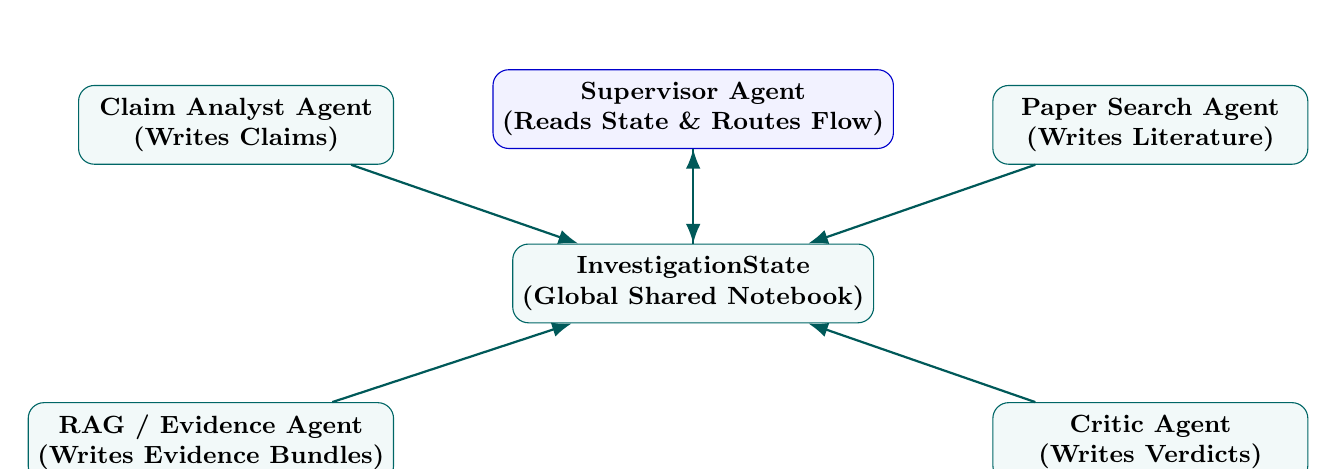
\begin{tikzpicture}[
    node distance=10mm and 15mm,
    statebox/.style={rectangle, draw=teal!80!black, fill=teal!5, rounded corners=2mm, minimum width=4cm, minimum height=1cm, align=center, font=\small\bfseries},
    arrow/.style={-{Latex[length=2.5mm]}, thick, draw=teal!70!black}
]
\node[statebox] (state) {InvestigationState\\(Global Shared Notebook)};
\node[statebox, above left=of state] (analyst) {Claim Analyst Agent\\(Writes Claims)};
\node[statebox, above right=of state] (search) {Paper Search Agent\\(Writes Literature)};
\node[statebox, below left=of state] (rag) {RAG / Evidence Agent\\(Writes Evidence Bundles)};
\node[statebox, below right=of state] (critic) {Critic Agent\\(Writes Verdicts)};
\node[statebox, above=12mm of state, draw=blue!80!black, fill=blue!5] (supervisor) {Supervisor Agent\\(Reads State \& Routes Flow)};

\draw[arrow] (analyst) -- (state);
\draw[arrow] (search) -- (state);
\draw[arrow] (rag) -- (state);
\draw[arrow] (critic) -- (state);
\draw[arrow, dashed] (supervisor) -- (state);
\draw[arrow] (state) -- (supervisor);
\end{tikzpicture}
\caption{State interaction diagram showing agents updating the shared notebook.}
\end{figure}

\subsection{\texttt{InvestigationState} Specification}
\begin{itemize}[leftmargin=*]
    \item \textbf{File:} \texttt{src/mascv/core/state.py}
    \item \textbf{Attributes:}
    \begin{itemize}
        \item \texttt{paper: Optional[ResearchPaper]}: Structured representation of the target paper.
        \item \texttt{claims: Dict[str, ClaimInvestigationState]}: Mapping of claim IDs (e.g. \texttt{C1}, \texttt{C2}) to their individual lifecycle progress.
        \item \texttt{active\_claim\_id: Optional[str]}: The specific claim currently being investigated by the active cycle.
        \item \texttt{system\_iteration: int}: Counter tracking how many feedback loops have occurred.
        \item \texttt{max\_iterations: int}: Hard upper bound (default 3) preventing infinite loops.
        \item \texttt{metadata: Dict[str, Any]}: Diagnostic store housing timing logs and routing decisions.
    \end{itemize}
\end{itemize}

% ==================================================
\section{Agent 1: Supervisor Agent}
% ==================================================

\begin{agentbox}{Supervisor Agent Summary}
\textbf{Core Question:} \textit{``What should the system do next?''}\\
\textbf{Primary Role:} System orchestrator, state monitor, iteration regulator, and adaptive router.\\
\textbf{Implementation Files:} \texttt{src/mascv/agents/supervisor.py}, \texttt{config/agents/supervisor.yaml}, \texttt{tests/unit/test\_agents/test\_supervisor.py}
\end{agentbox}

\subsection{Theoretical Purpose}
Without a Supervisor, multi-agent systems devolve into rigid, linear pipelines. However, scientific literature analysis is intrinsically non-linear: some claims enjoy abundant replication papers and can be finalized immediately, whereas other claims encounter conflicting evidence and require secondary literature discovery. The Supervisor evaluates uncertainty and controls workflow dispatching.

\subsection{Code Architecture: \texttt{src/mascv/agents/supervisor.py}}
\begin{itemize}[leftmargin=*]
    \item \textbf{Class:} \texttt{SupervisorAgent(BaseAgent)}
    \item \textbf{Key Method: \texttt{decide\_next\_step(state: InvestigationState) -> str}}
    Executes a deterministic four-tier decision tree:
    \begin{enumerate}
        \item \textit{Claim Existence Check:} If \texttt{state.claims} is empty and paper text is present, return \texttt{"claim\_analyst"}.
        \item \textit{Iteration Ceiling Check:} If \texttt{state.system\_iteration >= state.max\_iterations}, return \texttt{"finalize"}.
        \item \textit{Unprocessed Claim Check:} If any claim lacks external literature (\texttt{external\_papers\_found == []}), assign \texttt{state.active\_claim\_id} and return \texttt{"paper\_search"}.
        \item \textit{Feedback Loop Trigger:} If a claim has status \texttt{ClaimStatus.NEEDS\_MORE\_EVIDENCE} and is within the cycle limit, trigger \texttt{"paper\_search"} again.
        \item \textit{Completion:} When all claims are evaluated, return \texttt{"finalize"}.
    \end{enumerate}
\end{itemize}

\subsection{Configuration File: \texttt{config/agents/supervisor.yaml}}
\begin{lstlisting}
agent:
  name: "SupervisorAgent"
  model: "gemma-4-31b-it"
  temperature: 0.1
  parameters:
    max_search_cycles: 3
    min_confidence_to_finalize: 0.70
    min_independent_sources: 2
\end{lstlisting}

% ==================================================
\section{Agent 2: Claim Analyst Agent}
% ==================================================

\begin{agentbox}{Claim Analyst Summary}
\textbf{Core Question:} \textit{``What exactly are the authors claiming?''}\\
\textbf{Primary Role:} Filters academic discourse, isolates novel empirical contributions, and normalizes them into structured propositions.\\
\textbf{Implementation Files:} \texttt{src/mascv/agents/claim\_analyst.py}, \texttt{src/mascv/models/claim.py}, \texttt{config/agents/claim\_analyst.yaml}
\end{agentbox}

\subsection{Theoretical Purpose}
Scientific papers contain thousands of statements, including background reviews, standard mathematical definitions, and established axioms. Investigating non-novel statements wastes computational budget. The Claim Analyst isolates the primary testable contributions and converts vague textual declarations into normalized scientific propositions.

\subsection{Data Model: \texttt{src/mascv/models/claim.py}}
\begin{lstlisting}[language=Python]
class ClaimType(str, Enum):
    PERFORMANCE = "performance"       # Outperforms baseline accuracy/speed
    EFFICIENCY = "efficiency"         # Reduces FLOPs, memory, parameters
    CAUSAL = "causal"                 # Component X causes phenomenon Y
    GENERALIZATION = "generalization" # Holds across multiple domains
    METHODOLOGICAL = "methodological" # Novel algorithmic formulation
    NOVELTY = "novelty"               # First to propose mechanism

class Claim(BaseModel):
    id: str                           # Unique ID (e.g. C1, C2)
    paper_id: str                     # Source document identifier
    subject: str                      # Proposed method / algorithm
    statement: str                    # Normalized claim sentence
    claim_type: ClaimType             # Proposition classification
    benchmarks: List[str]             # Evaluation datasets
    metrics: List[str]                # Quantitative metrics
    comparisons: List[str]            # Prior baselines compared against
    conditions: Optional[str] = None  # Training setup / hardware limits
    status: ClaimStatus               # Lifecycle status (EXTRACTED, etc.)
\end{lstlisting}

% ==================================================
\section{Agent 3: Paper Search Agent}
% ==================================================

\begin{agentbox}{Paper Search Agent Summary}
\textbf{Core Question:} \textit{``What broader literature exists regarding this claim?''}\\
\textbf{Primary Role:} Discovers external academic literature using paired adversarial search queries.\\
\textbf{Implementation Files:} \texttt{src/mascv/agents/paper\_search.py}, \texttt{src/mascv/search/query\_generator.py}, \texttt{src/mascv/search/academic\_search/}
\end{agentbox}

\subsection{Adversarial Search Philosophy}
Standard information retrieval exhibits severe \textbf{confirmation bias}: searching only for positive terms (e.g. \textit{``Transformer achieves state of the art''}) returns only approving studies. The Paper Search Agent actively executes paired adversarial queries:
\begin{itemize}[leftmargin=*]
    \item \textbf{Supporting Queries:} Focus on replication, validation, and benchmark superiority (\textit{``Transformer translation replication''}, \textit{``Transformer BLEU benchmark''}).
    \item \textbf{Adversarial Queries:} Focus on limits, failures, and computational disparities (\textit{``Transformer failure cases''}, \textit{``Transformer computational limits''}, \textit{``Transformer benchmark leakage''}).
\end{itemize}

\subsection{Academic Connectors (\texttt{src/mascv/search/})}
\begin{itemize}[leftmargin=*]
    \item \texttt{academic\_search/arxiv\_client.py}: Queries the official arXiv REST API for preprints.
    \item \texttt{academic\_search/semantic\_scholar\_client.py}: Queries the Semantic Scholar Graph API for peer-reviewed citations, DOIs, and citation counts.
    \item \texttt{academic\_search/crossref\_client.py}: Discovers DOI metadata and publisher records.
\end{itemize}

% ==================================================
\section{Agent 4: RAG / Evidence Agent}
% ==================================================

\begin{agentbox}{RAG / Evidence Agent Summary}
\textbf{Core Question:} \textit{``What specific evidence inside these papers is relevant?''}\\
\textbf{Primary Role:} Parses multi-column PDFs, performs claim-aware chunking, and constructs structured Evidence Bundles.\\
\textbf{Implementation Files:} \texttt{src/mascv/agents/evidence\_rag.py}, \texttt{src/mascv/rag/parsers/}, \texttt{src/mascv/rag/chunking/}, \texttt{src/mascv/rag/evidence\_bundler.py}
\end{agentbox}

\subsection{Why Naive Token Chunking Fails}
Standard RAG systems slice documents into fixed token windows (e.g. 512 tokens). In scientific papers, a single empirical result is spread across multiple sections:
\begin{equation}
\text{Evidence} = \text{Methodology (Sec 3)} + \text{Hardware Setup (Sec 4)} + \text{Table 2 Result} + \text{Limitations Note (Sec 5)}
\end{equation}
Fixed chunking cuts this evidence in half. The RAG Agent instead uses \textbf{Claim-Aware Agentic Chunking} to assemble related components into an \textbf{Evidence Bundle}.

\subsection{The Evidence Bundle Data Structure (\texttt{src/mascv/models/evidence.py})}
\begin{lstlisting}[language=Python]
class EvidenceRelationship(str, Enum):
    SUPPORTS = "SUPPORTS"
    CONTRADICTS = "CONTRADICTS"
    QUALIFIES = "QUALIFIES"
    REPLICATES = "REPLICATES"
    CHALLENGES = "CHALLENGES"
    ALTERNATIVE = "ALTERNATIVE"

class EvidenceBundle(BaseModel):
    id: str
    claim_id: str
    source_paper_id: str
    source_title: str
    location: str                    # e.g., "Page 7, Table 2"
    content: str                     # Quantitative statement or excerpt
    context: Optional[str]           # Dataset, epoch budget, metric
    relationship: EvidenceRelationship
    confidence_score: float
\end{lstlisting}

% ==================================================
\section{Agent 5: Support Agent (The Proponent)}
% ==================================================

\begin{agentbox}{Support Agent Summary}
\textbf{Core Question:} \textit{``Why might this claim be true?''}\\
\textbf{Primary Role:} Constructs the strongest possible evidence-grounded affirmative argument.\\
\textbf{Implementation Files:} \texttt{src/mascv/agents/support\_agent.py}, \texttt{config/agents/support\_agent.yaml}
\end{agentbox}

\subsection{Responsibilities}
The Support Agent acts as the defense counsel. It reviews all evidence tagged with \texttt{SUPPORTS} or \texttt{REPLICATES} and synthesizes a logically connected case:
\begin{enumerate}
    \item Identifies independent replications across distinct research labs.
    \item Highlights ablation studies confirming that the proposed component caused the improvement.
    \item Explicitly links every premise to an \texttt{evidence\_id} in the Evidence Store.
\end{enumerate}

% ==================================================
\section{Agent 6: Attack Agent (The Adversary)}
% ==================================================

\begin{agentbox}{Attack Agent Summary}
\textbf{Core Question:} \textit{``Why might this claim be wrong, overstated, or conditional?''}\\
\textbf{Primary Role:} Uncovers experimental flaws, hidden computational budgets, and contradictory literature.\\
\textbf{Implementation Files:} \texttt{src/mascv/agents/attack\_agent.py}, \texttt{config/agents/attack\_agent.yaml}
\end{agentbox}

\subsection{Vulnerability Dimensions Probed}
The Attack Agent is an independent adversary. It investigates:
\begin{itemize}[leftmargin=*]
    \item \textbf{Computational Disparity:} Did the proposed method only win because it was trained with $10\times$ more compute?
    \item \textbf{Benchmark Contamination:} Was the evaluation dataset accidentally present in the pretraining corpus?
    \item \textbf{Failed Replications:} Are there external studies reporting lower or negligible gains?
    \item \textbf{Overgeneralization:} Did the authors claim general superiority while evaluating on only one dataset?
\end{itemize}

% ==================================================
\section{Agent 7: Critic Agent (The Scientific Judge)}
% ==================================================

\begin{agentbox}{Critic Agent Summary}
\textbf{Core Question:} \textit{``Which evidence and arguments actually hold up?''}\\
\textbf{Primary Role:} Validates citations, detects fallacies, and delivers the final scientific verdict.\\
\textbf{Implementation Files:} \texttt{src/mascv/agents/critic\_agent.py}, \texttt{src/mascv/models/verdict.py}
\end{agentbox}

\subsection{Four Judicial Validation Checks}
\begin{enumerate}[leftmargin=*]
    \item \textbf{Citation Grounding Check:} Does the primary source text actually support what the Support or Attack agent claimed it says?
    \item \textbf{Experimental Parity Check:} Were baseline models given equivalent tuning budgets?
    \item \textbf{Generalization Check:} Flags claims whose scope exceeds the experimental evidence.
    \item \textbf{Verdict Classification:} Assigns one of four definitive verdicts:
    \begin{itemize}
        \item \textbf{\texttt{Supported}:} Robust, replicated affirmative evidence under fair conditions.
        \item \textbf{\texttt{Partially Supported}:} Valid only under specific experimental constraints.
        \item \textbf{\texttt{Unsupported}:} Directly contradicted by reputable literature or fundamentally flawed.
        \item \textbf{\texttt{Inconclusive}:} Available literature is sparse, inaccessible, or unresolved.
    \end{itemize}
\end{enumerate}

% ==================================================
\section{Evaluation Framework \& Baselines}
% ==================================================

A graduation project must demonstrate empirical superiority over baselines. The \texttt{src/mascv/evaluation/} package implements:

\subsection{Baselines (\texttt{evaluation/baselines/})}
\begin{itemize}[leftmargin=*]
    \item \textbf{Baseline 1 (\texttt{single\_agent\_baseline.py}):} Single monolithic LLM with direct search tools.
    \item \textbf{Baseline 2 (\texttt{standard\_rag\_baseline.py}):} Conventional sliding-window chunking (512 tokens) without claim-aware bundling.
\end{itemize}

\subsection{Ablation Matrix (\texttt{evaluation/ablations/})}
Eight progressive configurations isolating every agentic contribution:
\begin{enumerate}
    \item Single LLM (No search, no RAG)
    \item Single Agent + Search Only
    \item Single Agent + RAG Only
    \item Fixed-Size Chunking RAG
    \item Claim-Aware Agentic RAG
    \item Support + Attack (No Critic)
    \item Support + Attack + Critic (Static pipeline, no Supervisor loop)
    \item \textbf{Full MASCV Multi-Agent System (Cyclical state graph)}
\end{enumerate}

% ==================================================
\section{Complete File Map \& Guide}
% ==================================================

\begingroup
\sloppy
\begin{longtable}{p{6.0cm} p{9.0cm}}
\toprule
\textbf{File Path} & \textbf{Precise Responsibility} \\
\midrule
\endhead
\path{src/mascv/models/paper.py} & Data schemas for parsed research papers, sections, and metadata. \\
\path{src/mascv/models/claim.py} & Data schemas for normalized claims and \texttt{ClaimStatus} enums. \\
\path{src/mascv/models/evidence.py} & Schemas for \texttt{EvidenceBundle} and evidence relationship tags. \\
\path{src/mascv/models/argument.py} & Schemas for proponent and opponent debate arguments. \\
\path{src/mascv/models/verdict.py} & Schemas for final verdicts, critic findings, and complete reports. \\
\path{src/mascv/core/state.py} & \texttt{InvestigationState} shared notebook schema. \\
\path{src/mascv/core/workflow.py} & LangGraph cyclical state graph linking agents. \\
\path{src/mascv/core/exceptions.py} & Project-wide custom exception classes. \\
\path{src/mascv/agents/base.py} & Abstract base class defining \texttt{execute()} interface. \\
\path{src/mascv/agents/supervisor.py} & State router, loop manager, and confidence checker. \\
\path{src/mascv/agents/claim_analyst.py} & Extracts and normalizes empirical claims using Gemma. \\
\path{src/mascv/agents/paper_search.py} & Adversarial literature discovery coordinator. \\
\path{src/mascv/agents/evidence_rag.py} & Extracts claim-aware evidence units from papers. \\
\path{src/mascv/agents/support_agent.py} & Builds affirmative evidence-grounded arguments. \\
\path{src/mascv/agents/attack_agent.py} & Builds adversarial counterarguments and limitation analyses. \\
\path{src/mascv/agents/critic_agent.py} & Validates citations and determines final verdict. \\
\path{src/mascv/search/query_generator.py} & Generates paired supporting and adversarial search queries. \\
\path{src/mascv/search/academic_search/arxiv_client.py} & arXiv API client for preprint discovery. \\
\path{src/mascv/search/academic_search/semantic_scholar_client.py} & Semantic Scholar API client for citation graph analysis. \\
\path{src/mascv/storage/evidence_store.py} & Repository housing all discovered evidence bundles. \\
\path{src/mascv/storage/provenance_graph.py} & Lineage graph tracking $\text{Claim} \rightarrow \text{Source}$. \\
\path{src/mascv/utils/llm.py} & Unified LLM client for Gemma 4 31B and Pydantic JSON parsing. \\
\path{ui/frontend/streamlit_app.py} & Interactive multi-page Streamlit web dashboard. \\
\bottomrule
\end{longtable}
\endgroup

\end{document}
